Commençons par noter que la méthode \quote{on avance au mieux} n'est pas la plus efficace possible comme le montre l'exemple suivant où six mouvements totalement inutiles sont effectués si bien que l'on n'a toujours pas gagné à la neuvième étape 
\footnote{
	En fait, il faut $39$ mouvements pour gagner avec la méthode \quote{on avance au mieux}, et la méthode \quote{une base à la fois} en demande $25$.
}. Il est important de noter ici que nous appliquons à la lettre les mouvements demandés par l'algorithme ! Il est sûrement évident pour le lecteur de voir l'inutilité des tous premiers mouvements.

\vspace{-0.4em}
\begin{multicols}{2}
	\begin{center}   % [4, 4, None, 0, 1, 1, 2, 2, 3, 3]
		\includegraphics[scale= 0.45]{content/optimal/where_do_we_go/algo_bubble/000.png}

		\includegraphics[scale= 0.45]{content/optimal/where_do_we_go/algo_bubble/001.png}

		\includegraphics[scale= 0.45]{content/optimal/where_do_we_go/algo_bubble/002.png}

		\includegraphics[scale= 0.45]{content/optimal/where_do_we_go/algo_bubble/003.png}

		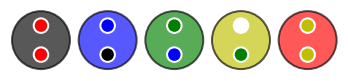
\includegraphics[scale= 0.45]{content/optimal/where_do_we_go/algo_bubble/004.png}
	\end{center}

	\columnbreak
	\begin{center}   % [4, 4, None, 0, 1, 1, 2, 2, 3, 3]
		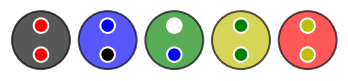
\includegraphics[scale= 0.45]{content/optimal/where_do_we_go/algo_bubble/005.png}

		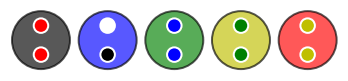
\includegraphics[scale= 0.45]{content/optimal/where_do_we_go/algo_bubble/006.png}

		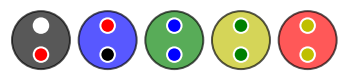
\includegraphics[scale= 0.45]{content/optimal/where_do_we_go/algo_bubble/007.png}

		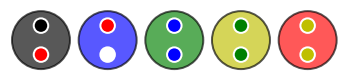
\includegraphics[scale= 0.45]{content/optimal/where_do_we_go/algo_bubble/008.png}

		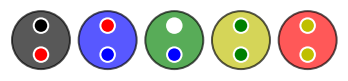
\includegraphics[scale= 0.45]{content/optimal/where_do_we_go/algo_bubble/009.png}
	\end{center}
\end{multicols}


\medskip

Ici, on peut gagner en seulement 9 coups ! Voici les mouvements à faire
\footnote{
	Notez au passage les enseignements que l'on peut tirer d'une configuration très, très particulière.
}.
Nous verrons bientôt que l'on ne peut pas faire mieux.

\vspace{-0.4em}
\begin{multicols}{2}
	\begin{center}   % [4, 4, None, 0, 1, 1, 2, 2, 3, 3]
		\includegraphics[scale= 0.45]{content/optimal/where_do_we_go/tree_sol/000.png}

		\includegraphics[scale= 0.45]{content/optimal/where_do_we_go/tree_sol/001.png}

		\includegraphics[scale= 0.45]{content/optimal/where_do_we_go/tree_sol/002.png}

		\includegraphics[scale= 0.45]{content/optimal/where_do_we_go/tree_sol/003.png}

		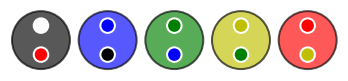
\includegraphics[scale= 0.45]{content/optimal/where_do_we_go/tree_sol/004.png}
	\end{center}

	\columnbreak
	\begin{center}   % [4, 4, None, 0, 1, 1, 2, 2, 3, 3]
		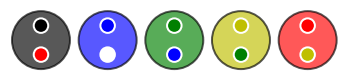
\includegraphics[scale= 0.45]{content/optimal/where_do_we_go/tree_sol/005.png}

		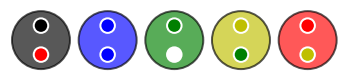
\includegraphics[scale= 0.45]{content/optimal/where_do_we_go/tree_sol/006.png}

		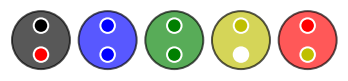
\includegraphics[scale= 0.45]{content/optimal/where_do_we_go/tree_sol/007.png}

		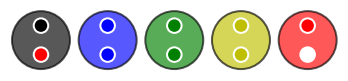
\includegraphics[scale= 0.45]{content/optimal/where_do_we_go/tree_sol/008.png}

		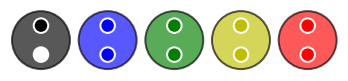
\includegraphics[scale= 0.45]{content/optimal/where_do_we_go/tree_sol/009.png}
	\end{center}
\end{multicols}


\medskip

Précisions ce que nous cherchons à faire : nous voulons trouver une solution peu coûteuse. Très bien ! Mais dans ce cas, comment évalue-t-on ce coût ? Nous choisissons de chercher à minimiser le nombre de déplacements du trou (donc toute opération autre que le déplacement d'un jeton ne sera pas comptabilisée).
Dans le premier cas ci-dessus, le coût est strictement plus grand que $9$, tandis que pour le second, il vaut exactement $9$. La section suivante va proposer un algorithme donnant à coup sûr la solution la moins coûteuse.
